% gr-Coxeter.tex -- the Coxeter graph : 28 vertices, 42 edges, cubic,
% girth 7, not Hamiltonian. Three 7-cycles a (step 1), b (step 2),
% c (step 3) on a circle, and d_i joined to a_i, b_i, c_i.
% Engine : pdfLaTeX or LuaLaTeX
\documentclass[border=3mm, convert=false]{standalone}
\usepackage{tkz-berge}
\begin{document}
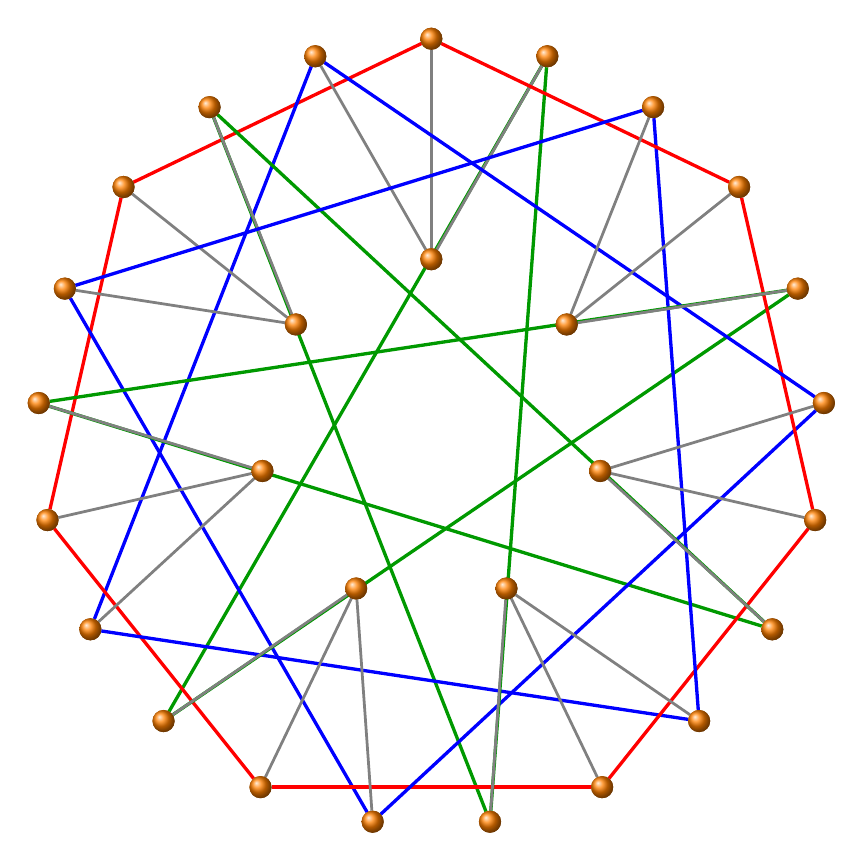
\begin{tikzpicture}
  \GraphInit[vstyle=Art]
  \SetVertexNoLabel
  \tikzset{VertexStyle/.append style = {minimum size = 8pt}}
  \foreach \i in {0,...,6}{%
    \pgfmathsetmacro\t{90+360*\i/7}
    \Vertex[a=\t,d=5]{a\i}
    \Vertex[a=\t+360/21,d=5]{b\i}
    \Vertex[a=\t-360/21,d=5]{c\i}
    \Vertex[a=\t,d=2.2]{d\i}}
  \foreach \i in {0,...,6}{%
    \pgfmathtruncatemacro\p{mod(\i+1,7)}
    \pgfmathtruncatemacro\q{mod(\i+2,7)}
    \pgfmathtruncatemacro\r{mod(\i+3,7)}
    \Edge[local,color=red,lw=1.2pt](a\i)(a\p)
    \Edge[local,color=blue,lw=1.2pt](b\i)(b\q)
    \Edge[local,color=green!60!black,lw=1.2pt](c\i)(c\r)
    \foreach \v in {a,b,c}{\Edge[local,color=gray,lw=1pt](d\i)(\v\i)}}
  \foreach \i in {0,...,6}{\foreach \v in {a,b,c,d}{\Vertex[Node]{\v\i}}}
\end{tikzpicture}
\end{document}
